% SC3010 --- Chapter 1: Foundations of Computer Security (0->100 ground-up)
\chapter{Foundations: CIA Triad, Threats, Risk and Attack Surfaces}
\label{ch:foundation}

\begin{quote}
\emph{``Security is a process, not a product.''} --- Bruce Schneier. Before we encrypt anything we must agree on what we are protecting, from whom, at what cost, and where the doors are.
\end{quote}

\noindent\fbox{\parbox{\dimexpr\linewidth-2\fboxsep-2\fboxrule}{%
\textbf{From zero: no prior security knowledge assumed.} We build from everyday intuition---a locked diary, a tampered letter, a shop that must stay open---to formal definitions of confidentiality, integrity and availability. Every term is defined on first use. This chapter is the vocabulary for the whole book.}}
\vspace{0.4em}

\section*{Learning Outcomes}
After this chapter you will be able to:
\begin{enumerate}[label=(L\arabic*)]
    \item state the CIA triad and classify a security requirement under C, I or A;
    \item distinguish threat, vulnerability, attack and exploit with examples;
    \item apply STRIDE to enumerate threats for a simple system;
    \item compute and prioritise risk as likelihood $\times$ impact (qualitative and quantitative);
    \item identify and reduce the attack surface of a system across network, software, human and physical layers.
\end{enumerate}

% ============================================================
\section{What Are We Protecting? The CIA Triad}
\label{sec:cia}
Intuition first. A diary has three wishes: nobody else reads it (secrecy), nobody rewrites a page without you noticing (accuracy), and you can open it when you want (reachability). Computer security generalises these to \emph{confidentiality}, \emph{integrity} and \emph{availability}---the CIA triad. Almost every requirement maps to one or more of them.

\begin{figure}[h]
\centering
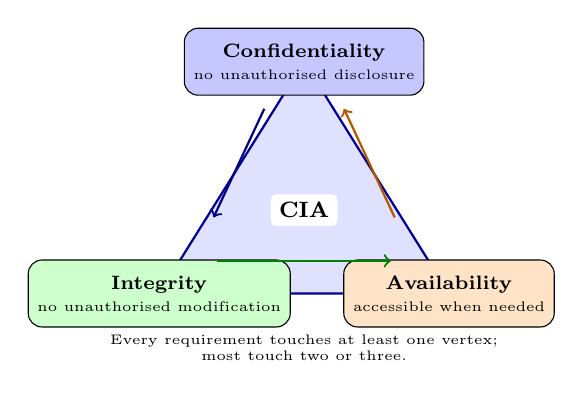
\begin{tikzpicture}[scale=0.92,every node/.style={font=\scriptsize}]
  \coordinate (C) at (0,2.2); \coordinate (I) at (-2.0,-1.0); \coordinate (A) at (2.0,-1.0);
  \fill[blue!12,draw=blue!60!black,thick,rounded corners=4pt] (C) -- (I) -- (A) -- cycle;
  \node[draw,fill=blue!22,rounded corners=5pt,minimum width=2.3cm,minimum height=0.85cm,align=center] at (C) {\textbf{Confidentiality}\\\tiny no unauthorised disclosure};
  \node[draw,fill=green!20,rounded corners=5pt,minimum width=2.3cm,minimum height=0.85cm,align=center] at (I) {\textbf{Integrity}\\\tiny no unauthorised modification};
  \node[draw,fill=orange!22,rounded corners=5pt,minimum width=2.3cm,minimum height=0.85cm,align=center] at (A) {\textbf{Availability}\\\tiny accessible when needed};
  \node[font=\footnotesize\bfseries,fill=white,rounded corners=2pt,inner sep=3pt] at (0,0.15) {CIA};
  \draw[->,thick,blue!50!black] (-0.55,1.55) -- (-1.25,0.05);
  \draw[->,thick,green!50!black] (-1.2,-0.55) -- (1.2,-0.55);
  \draw[->,thick,orange!70!black] (1.25,0.05) -- (0.55,1.55);
  \node[font=\tiny,align=center] at (0,-1.75) {Every requirement touches at least one vertex;\\most touch two or three.};
\end{tikzpicture}
\caption{The CIA triad. Confidentiality protects disclosure, integrity protects modification, availability protects access. Tension between them drives design trade-offs.}
\label{fig:cia}
\end{figure}

\begin{definition}[CIA triad]
\begin{itemize}[leftmargin=1.2em,itemsep=0.25em]
    \item \textbf{Confidentiality:} information is not disclosed to unauthorised entities. Enforced by access control, encryption, least privilege.
    \item \textbf{Integrity:} information and systems are not altered in an unauthorised or undetectable way. Covers data integrity and origin authenticity. Enforced by hashes, MACs, signatures.
    \item \textbf{Availability:} authorised users can access information and services when needed. Enforced by redundancy, rate-limiting, DoS mitigation.
\end{itemize}
\end{definition}

Overlap is normal. A signed software update needs integrity (not tampered) \emph{and} authenticity (from the vendor, hence confidentiality of the signing key) \emph{and} availability (patch must arrive). Two later refinements appear often: \emph{authenticity} and \emph{non-repudiation} are usually treated as facets of integrity; \emph{accountability} spans all three via logging.

\begin{example}[Classifying requirements]
Online exam: (a) student A cannot see student B's answers --- confidentiality; (b) submitted answers cannot be altered after deadline --- integrity; (c) submission portal stays up during the window --- availability. Encrypting the database helps (a) but does not help (c).
\end{example}

Trade-offs matter. Requiring a 20-character password and hardware token improves confidentiality but can hurt availability (users locked out) and even integrity (users write passwords on sticky notes). Good security balances the triangle for the asset at hand.

% ============================================================
\section{Threats, Vulnerabilities, Attacks}
\label{sec:threats}
Picture a house: a burglar who wants jewellery is the \emph{threat actor}, an unlocked window is the \emph{vulnerability}, climbing in is the \emph{attack}, the crowbar used is the \emph{exploit}, and the jewellery is the \emph{asset}. Security language follows the same chain.

\begin{definition}[Core terms]
An \textbf{asset} is what we value (data, service, reputation). A \textbf{vulnerability} is a weakness that can be exploited (bug, misconfiguration, human habit). A \textbf{threat} is a potential event that could harm an asset via a vulnerability. A \textbf{threat actor} is who or what carries it out (insider, criminal, nation-state, botnet). An \textbf{attack} is the realised threat; an \textbf{exploit} is the concrete technique or code.
\end{definition}

\begin{figure}[h]
\centering
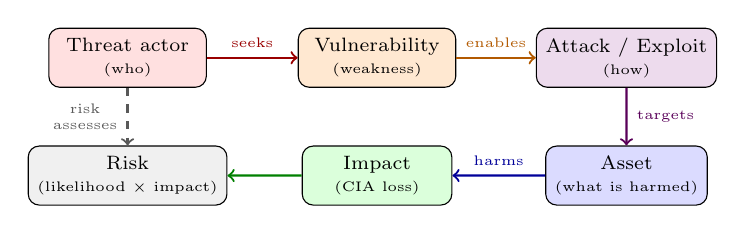
\begin{tikzpicture}[every node/.style={font=\scriptsize},scale=0.88]
  \node[draw,fill=red!12,rounded corners=4pt,minimum width=2.0cm,minimum height=0.75cm,align=center] (threat) at (0,0) {Threat actor\\\tiny (who)};
  \node[draw,fill=orange!18,rounded corners=4pt,minimum width=2.0cm,minimum height=0.75cm,align=center] (vuln) at (3.6,0) {Vulnerability\\\tiny (weakness)};
  \node[draw,fill=violet!14,rounded corners=4pt,minimum width=2.0cm,minimum height=0.75cm,align=center] (attack) at (7.2,0) {Attack / Exploit\\\tiny (how)};
  \node[draw,fill=blue!14,rounded corners=4pt,minimum width=1.9cm,minimum height=0.75cm,align=center] (asset) at (7.2,-1.7) {Asset\\\tiny (what is harmed)};
  \node[draw,fill=green!14,rounded corners=4pt,minimum width=1.9cm,minimum height=0.75cm,align=center] (impact) at (3.6,-1.7) {Impact\\\tiny (CIA loss)};
  \node[draw,fill=gray!12,rounded corners=4pt,minimum width=1.9cm,minimum height=0.75cm,align=center] (risk) at (0,-1.7) {Risk\\\tiny (likelihood $\times$ impact)};
  \draw[->,thick,red!60!black] (threat) -- (vuln) node[midway,above,font=\tiny] {seeks};
  \draw[->,thick,orange!70!black] (vuln) -- (attack) node[midway,above,font=\tiny] {enables};
  \draw[->,thick,violet!70!black] (attack) -- (asset) node[midway,right,font=\tiny] {targets};
  \draw[->,thick,blue!60!black] (asset) -- (impact) node[midway,above,font=\tiny] {harms};
  \draw[->,thick,green!50!black] (impact) -- (risk);
  \draw[->,thick,gray!70!black,dashed] (threat) -- (risk) node[midway,left,font=\tiny,align=center] {risk\\assesses};
\end{tikzpicture}
\caption{From actor to risk: a threat actor exploits a vulnerability to attack an asset, causing an impact measured as risk.}
\label{fig:threat-chain}
\end{figure}

Enumerating threats systematically helps. \textbf{STRIDE} (Microsoft) asks six questions per component: \textbf{S}poofing (authenticity), \textbf{T}ampering (integrity), \textbf{R}epudiation (non-repudiation), \textbf{I}nformation disclosure (confidentiality), \textbf{D}enial of service (availability), \textbf{E}levation of privilege (authorisation). Walk each data flow and store through STRIDE and you rarely miss a class.

\begin{example}[STRIDE on a file upload]
Upload endpoint: spoofing --- attacker impersonates a user via stolen cookie; tampering --- modifies file in transit; repudiation --- denies uploading malware; information disclosure --- reads other users' files via path traversal; DoS --- uploads huge files to fill disk; elevation --- uploads a web shell to gain server execution. One feature, six lenses.
\end{example}

We also distinguish \emph{attack vectors} (path in: network, USB, phishing email) from \emph{attack surfaces} (next section).

\begin{remark}[Threat modelling steps]
A lightweight workflow: (1) draw the data-flow diagram, (2) walk each element through STRIDE, (3) score each threat by risk, (4) decide mitigate/transfer/accept/avoid, (5) record residual risk and review after changes. Tools like OWASP Threat Dragon automate (1)--(3) but judgement in (4) remains human.
\end{remark}

\begin{example}[STRIDE on a login form]
Login: spoofing --- credential stuffing with leaked passwords; tampering --- parameter tampering on \texttt{next} URL to phish; repudiation --- attacker denies brute-force attempts without logs; information disclosure --- verbose ``user exists'' errors enumerate accounts; DoS --- rate-limit bypass locks accounts; elevation --- SQL injection in username field. Mitigations map directly: MFA, input validation, audit logging, generic errors, rate limiting, prepared statements.
\end{example}

% ============================================================
\section{Risk: Likelihood \texorpdfstring{$\times$}{x} Impact}
\label{sec:risk}
Not every threat deserves the same budget. \emph{Risk} lets us prioritise. Intuitively: how likely is it, and how bad if it happens?

\begin{definition}[Risk]
\textbf{Risk} is the expected loss from a threat exploiting a vulnerability. Qualitatively,
\begin{align}
\text{Risk} = \text{Likelihood} \times \text{Impact},
\label{eq:risk}
\end{align}
often scored on a matrix (e.g., $3\times 3$ or $5\times 5$). Quantitatively, annualised loss expectancy $\text{ALE}=\text{ARO}\times\text{SLE}$ where $\text{ARO}$ is annualised rate of occurrence and $\text{SLE}$ single loss expectancy.
\end{definition}

\begin{example}[ALE]
A phishing breach costs $\text{SLE}=\$80{,}000$ and occurs $\text{ARO}=0.3$/year without training. $\text{ALE}= \$24{,}000$/year. Training at $\$8{,}000$/year that halves $\text{ARO}$ to $0.15$ saves $\$12{,}000$ in ALE --- net benefit $\$4{,}000$.
\end{example}

\begin{lstlisting}[language=Python,caption={Risk register ranking (qualitative $5\times5$).},label={lst:risk}]
def risk_score(likelihood, impact):
    # both 1..5  -> 1..25
    assert 1 <= likelihood <= 5 and 1 <= impact <= 5
    return likelihood * impact

risks = [("SQLi on login", 4, 5), ("USB drop in lobby", 2, 4), ("CDN outage", 3, 3)]
for name, L, I in sorted(risks, key=lambda r: risk_score(r[1], r[2]), reverse=True):
    print(name, risk_score(L, I))
# SQLi=20 (critical), USB=8 (medium), CDN=9 (medium)
\end{lstlisting}

Risk handling has four options: \emph{mitigate} (patch, add control), \emph{transfer} (insurance, outsource), \emph{accept} (low risk, cost exceeds benefit), \emph{avoid} (remove the feature). Residual risk --- what remains after controls --- is what management signs off on. Threat modelling without risk ranking is just a wish list.

% ============================================================
\section{Attack Surfaces}
\label{sec:surface}
The \emph{attack surface} is the sum of all points where an attacker can interact with the system. Smaller surface, fewer places to be wrong.

\begin{figure}[h]
\centering
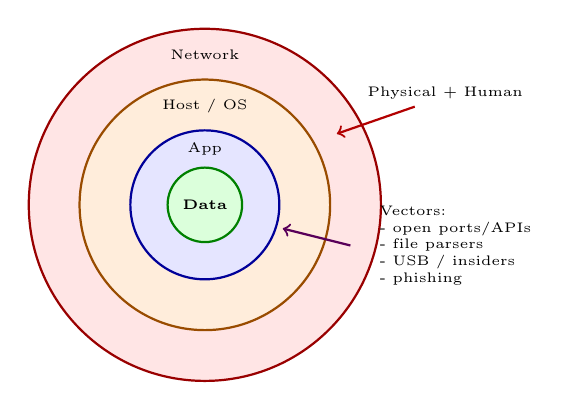
\begin{tikzpicture}[scale=0.86,every node/.style={font=\scriptsize}]
  \fill[red!10] (0,0) circle (2.6);
  \fill[orange!14] (0,0) circle (1.85);
  \fill[blue!10] (0,0) circle (1.1);
  \fill[green!14] (0,0) circle (0.55);
  \draw[thick,red!60!black] (0,0) circle (2.6);
  \draw[thick,orange!60!black] (0,0) circle (1.85);
  \draw[thick,blue!60!black] (0,0) circle (1.1);
  \draw[thick,green!50!black] (0,0) circle (0.55);
  \node[font=\tiny\bfseries,align=center] at (0,0) {Data};
  \node[font=\tiny,align=center] at (0,0.82) {App};
  \node[font=\tiny,align=center] at (0,1.46) {Host / OS};
  \node[font=\tiny,align=center] at (0,2.22) {Network};
  \node[font=\tiny,fill=white,rounded corners=2pt,inner sep=2pt] at (3.55,1.65) {Physical + Human};
  \draw[->,thick,red!70!black] (3.1,1.45) -- (1.95,1.05);
  \node[font=\tiny,align=left] at (3.7,-0.6) {Vectors:\\- open ports/APIs\\- file parsers\\- USB / insiders\\- phishing};
  \draw[->,thick,violet!70!black] (2.15,-0.6) -- (1.15,-0.35);
\end{tikzpicture}
\caption{Layered attack surface: network $\supset$ host $\supset$ application $\supset$ data, with human and physical vectors cutting across. Reducing surface means fewer exposed interfaces at each ring.}
\label{fig:surface}
\end{figure}

Dimensions to audit: \textbf{network} (open ports, APIs, protocols, wireless), \textbf{software} (input parsers, dependencies, plugins, debug endpoints), \textbf{human} (phishing susceptibility, insider actions, shadow IT), \textbf{physical} (USB ports, unlocked terminals, discarded drives). A classic reduction playbook: close unused ports, disable unused features and accounts, enforce least privilege, validate every input at the trust boundary, keep dependencies minimal and patched.

\begin{example}[Surface reduction]
A campus printer exposing Telnet, FTP, a web panel and mDNS has a network surface of four services. Disabling Telnet/FTP (unused), putting the panel behind VPN and SSO, and turning off mDNS outside the subnet cuts the reachable surface by three quarters without buying anything.
\end{example}

Attack surface analysis pairs with \emph{trust boundaries}: draw where data crosses from untrusted to trusted (browser $\to$ server, server $\to$ DB). Every crossing needs validation, authentication and logging.

% ============================================================
\section{Design Principles: Least Privilege and Defence in Depth}
\label{sec:principles}
Two principles guide every later chapter. \textbf{Least privilege} says each component gets only the permissions it needs and no more, for the shortest time needed. A PDF viewer that can launch PowerShell violates it; a web app running as root does too. Enforce via roles, capabilities, sandboxing and short-lived tokens.

\textbf{Defence in depth} (layered security) says no single control should be a single point of failure. An attacker who phishes a password still faces MFA; who bypasses MFA still faces network segmentation; who reaches the DB still faces encrypted rows and audit logs. Each layer assumes the outer one has already fallen.

Other Saltzer--Schroeder principles reinforce these: \emph{fail-safe defaults} (deny by default), \emph{complete mediation} (check every access), \emph{open design} (security must not depend on secrecy of the design), \emph{separation of duties} (no one person can both request and approve a wire transfer), \emph{least common mechanism} and \emph{psychological acceptability} (controls users can actually use).

\begin{definition}[Threat model]
A \textbf{threat model} is a structured description of what you defend, whom you defend against, and what you assume the attacker can and cannot do. It fixes scope: network attacker vs.\ local attacker, honest-but-curious vs.\ fully malicious, computational bounds, physical access.
\end{definition}

\begin{example}[Threat model matters]
Full-disk encryption protects against a stolen laptop (attacker gets disk, not key) but not against malware running while you are logged in (attacker is inside the trust boundary). Same tool, different model, different outcome. State the model before claiming ``secure.''
\end{example}

Risk, surface and principles together drive the security lifecycle: \emph{identify} assets and threats $\to$ \emph{assess} risk $\to$ \emph{mitigate} via layered, least-privilege controls that shrink the surface $\to$ \emph{verify} and \emph{monitor}.

\begin{remark}[Common pitfall]
``We encrypt, therefore we are secure'' ignores the model. Encryption without integrity invites padding-oracle attacks; availability without rate limits invites DoS; least privilege without audit invites insider misuse. Always ask \emph{which} CIA property, against \emph{which} threat model, at \emph{what} residual risk.
\end{remark}

% ============================================================
\section{Chapter Notes}
Further reading: Anderson's \emph{Security Engineering} (3rd ed.) for CIA trade-offs in real systems; NIST SP 800-30 for risk assessment and 800-154 for threat modelling. STRIDE is documented in Shostack's \emph{Threat Modeling: Designing for Security}. For attack surface metrics see Manadhata and Wing (2011). Common Criteria (ISO 15408) formalises the asset--threat--control vocabulary used here. Saltzer and Schroeder (1975) remains the classic on design principles---read Section~2 before any system design review.

% ============================================================
\section{Exercises}
\label{sec:ch01-exercises}
\begin{enumerate}[label=E1.\arabic*, leftmargin=*, itemsep=0.8em]
    \item \textbf{CIA classification.} For each, name the primary CIA property (and any secondary): (a) ransomware encrypts a hospital's records; (b) an attacker replays a captured payment request; (c) a CDN caches a private profile page; (d) a sensor sends stale temperature readings due to a dead battery. Justify in one sentence each.
    \item \textbf{Threat vs.\ vulnerability vs.\ attack.} Give concrete examples (one sentence each) showing they are distinct: a vulnerability with no known threat, a threat with no current vulnerability, and an attack that failed because the vulnerability had been patched. Explain why conflating them misallocates budget.
    \item \textbf{STRIDE walk.} Draw a data-flow diagram for a password-reset via email (browser $\to$ web app $\to$ mail server $\to$ browser). List one STRIDE threat per element/flow and state the CIA impact. Which two would you fix first and why?
    \item \textbf{Risk arithmetic.} Two risks: A has likelihood $4/5$ and impact $\$200{,}000$; B has likelihood $2/5$ and impact $\$500{,}000$. Compute expected loss for each. If a $\$30{,}000$ control halves B's likelihood, is it worthwhile? How does a $5\times5$ qualitative matrix ($L,I\in\{1..5\}$) change the ranking versus expected value?
    \item \textbf{Attack surface audit.} Pick a real system you use (e.g., your laptop, a lab router, or the NTU Learn app). Enumerate at least six attack-surface elements across network/software/human/physical, mark the trust boundaries, and propose three concrete reductions. Estimate before/after surface qualitatively.
\end{enumerate}
% End of Chapter 1
